%!TEX TS-program = xelatex

\documentclass[t]{beamer}  % [t], [c], или [b] --- вертикальное выравнивание на слайдах (верх, центр, низ)
%\documentclass[t, handout]{beamer} % Раздаточный материал (на слайдах всё сразу)
%\documentclass[aspectratio=169, t]{beamer} % Соотношение сторон

\usepackage{epstopdf}

%\usetheme{Berkeley} % Тема оформления
%\usetheme{Bergen}
%\usetheme{Szeged}

%\usecolortheme{beaver} % Цветовая схема
%\useinnertheme{circles}
%\useinnertheme{rectangles}

\usepackage{HSE-theme/beamerthemeHSE} % Подгружаем тему


%%% Работа с русским языком
\usepackage{cmap}					% поиск в PDF
\usepackage{mathtext} 				% русские буквы в формулах
\usepackage[T2A]{fontenc}			% кодировка
\usepackage[utf8]{inputenc}			% кодировка исходного текста
%%% Работа с русским языком и шрифтами
\usepackage[english,russian]{babel}   % загружает пакет многоязыковой вёрстки


%%% Дополнительная работа с математикой
\usepackage{amsmath,amsfonts,amssymb,amsthm,mathtools} % AMS
\usepackage{icomma} % "Умная" запятая: $0,2$ --- число, $0, 2$ --- перечисление

%% Номера формул
%\mathtoolsset{showonlyrefs=true} % Показывать номера только у тех формул, на которые есть \eqref{} в тексте.
%\usepackage{leqno} % Нумерация формул слева

%% Свои команды
\DeclareMathOperator{\sgn}{\mathop{sgn}}

%% Перенос знаков в формулах (по Львовскому)
\newcommand*{\hm}[1]{#1\nobreak\discretionary{}
	{\hbox{$\mathsurround=0pt #1$}}{}}

%%% Работа с картинками
\usepackage{graphicx}  % Для вставки рисунков
\graphicspath{{images/}{images2/}}  % папки с картинками
\setlength\fboxsep{3pt} % Отступ рамки \fbox{} от рисунка
\setlength\fboxrule{1pt} % Толщина линий рамки \fbox{}
\usepackage{wrapfig} % Обтекание рисунков текстом
\usepackage{caption}


%%% Работа с таблицами
\usepackage{array,tabularx,tabulary,booktabs} % Дополнительная работа с таблицами
\usepackage{longtable}  % Длинные таблицы
\usepackage{multirow} % Слияние строк в таблице

%%% Программирование
\usepackage{etoolbox} % логические операторы

%%% Другие пакеты
\usepackage{lastpage} % Узнать, сколько всего страниц в документе.
\usepackage{soul} % Модификаторы начертания
\usepackage{csquotes} % Еще инструменты для ссылок
%\usepackage[style=authoryear,maxcitenames=2,backend=biber,sorting=nty]{biblatex}
\usepackage{multicol} % Несколько колонок

%%% Картинки
\usepackage{tikz} % Работа с графикой
\usepackage{pgfplots}
\usepackage{pgfplotstable}
\usepackage{verbatim}
\usetikzlibrary{fadings}
\usepackage[outline]{contour}

\usepackage{chngcntr} % нумерация графиков и таблиц по секциям
\counterwithin{table}{section}
\counterwithin{figure}{section}

\usepackage{listings}

\lstdefinelanguage{Rust}{
  sensitive=true,
  morekeywords=[1]{
    break, continue, else, for, if, loop, match, return, while,
  },
  morekeywords=[2]{
    crate, fn, async, mod, pub, use, self, Self,
    struct, enum, const, static, let, mut, ref, type, impl,
    trait, where, as, dyn, move,
  },
  morekeywords=[3]{
    bool, char, i8, i16, i32, i64, isize, u8, u16, u32, u64, usize, f32, f64, str, String,
  },
  morekeywords=[4]{
    Ok, Err, Some, None,
  },
  morekeywords=[5]{
    await,
  },
  keywordstyle=[5]{\color{purple}},
  morecomment=[s]{/*}{*/},
  morecomment=[l]//,
  morestring=[b]",
  morestring=[b]r",
  morestring=[b]'',
}

\lstset{
  language=Rust,
  basicstyle=\ttfamily,
  keywordstyle=\color{blue},
  stringstyle=\color{red},
  commentstyle=\color{green},
  showstringspaces=false,
  breaklines=true,
  frame=none,
}


\lstnewenvironment{rustcode}[1][]{
  \lstset{
    language=Rust,
    basicstyle=\ttfamily,
    keywordstyle=\color{blue},
    stringstyle=\color{red},
    commentstyle=\color{gray},
    showstringspaces=false,
    breaklines=true,
    % frame=single,
    #1
  }
}{}

\usepackage{setspace}
\usepackage{color}


\title{Реализация поддержки асинхронного программирования для фреймворка \texttt{DSLab}}
\author{Артём Макогон}
\date{\today}
% \institute[Высшая школа экономики]{National Research University\\ 
	% <<Higher School of Economics>>}



\begin{document}
	
	\begin{frame}
		\maketitle
	\end{frame}
	

    \section{Введение}
    \subsection{Описание предметной области}

	\begin{frame}[fragile]
		\frametitle{\insertsection} 
		\framesubtitle{\insertsubsection}

		\begin{columns}
			\begin{column}{0.5\linewidth}
				\vspace{0.5cm}
				\begin{itemize}
					\item Большой объем данных/вычислений 
					\item Надежность
					\item Масштабируемость
				\end{itemize}
				\alt<2>{
					{ \hspace{2cm} \large $\Downarrow$ } 
					\begin{itemize}
						\item[\small\textgreater] Недетерминированные алгоритмы
						\item[\small\textgreater] Сложное тестирование
					\end{itemize}
				}{}
			\end{column}
			\begin{column}{0.6\linewidth}
				\vspace{1cm}
				
\includegraphics[width=\linewidth]{images/ds_intro}
			\end{column}
		\end{columns}
		
	\end{frame}

	\subsection{Дискретно-событийное моделирование}

    \begin{frame}
    \frametitle{\insertsection} 
	\framesubtitle{\insertsubsection}

	\begin{figure}
		\centering
		\includegraphics<1>[width=\linewidth]{images/event_pipeline_0}
		\includegraphics<2>[width=\linewidth]{images/event_pipeline_1}
		\includegraphics<3>[width=\linewidth]{images/event_pipeline_2}
		\includegraphics<4>[width=\linewidth]{images/event_pipeline_3}
		\includegraphics<5>[width=\linewidth]{images/event_pipeline_4}
		\includegraphics<6>[width=\linewidth]{images/event_pipeline_5}
		\includegraphics<7>[width=\linewidth]{images/event_pipeline_6}
		\includegraphics<8>[width=\linewidth]{images/event_pipeline_7}
		\includegraphics<9>[width=\linewidth]{images/event_pipeline_8}
		\includegraphics<10>[width=\linewidth]{images/event_pipeline_9}
		\label{simulation}
		\caption*{Исполнение симуляции}
	\end{figure}
        
    \end{frame}

	\subsection{Архитектура проекта \texttt{DSLab}}
	\begin{frame}
		\frametitle{\insertsection} 
		\framesubtitle{\insertsubsection}

		\begin{figure}[H]
			\centering
			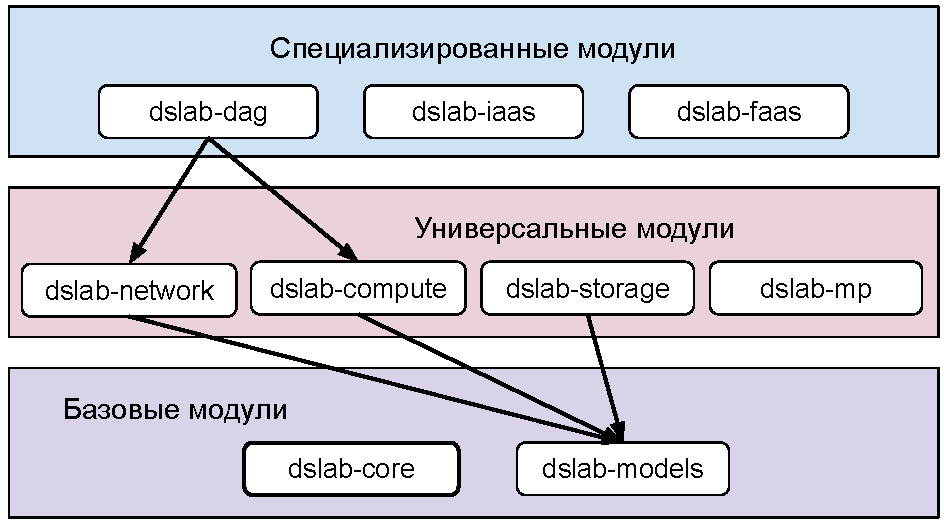
\includegraphics[width=0.9\linewidth]{images/dslab_arc}
			\caption*{Архитектура \texttt{DSLab}}
			\label{dslab_arc}
		\end{figure}
	\end{frame}


	\subsection{\texttt{Callback} модель. Реализация \texttt{Process}.}
	\begin{frame}[fragile]
		\frametitle{\insertsection} 
		\framesubtitle{\insertsubsection}
		\begin{columns}[c] 
			\begin{column}{0.73\textwidth} % First column
		\begin{figure}
			\scriptsize
			\centering
			\begin{rustcode}[escapeinside={(*@}{@*)}]
fn on(&mut self, event: Event) {
  cast!(match event.data {
    Start {} => {
      self.on_start(); (*@\tikz{\node[draw, fill=OldHSEblue, rounded corners, minimum width=1.5em, minimum height=1.5em] {};}@*)
    }
    DownloadCompleted {data} => {
      self.on_download_completed(data); (*@\tikz{\node[draw, fill=orange, rounded corners, minimum width=1.5em, minimum height=1.5em] {};}@*)
    }
    DiskWriteCompleted => {
      self.on_disk_write_completed(); (*@\tikz{\node[draw, fill=HSEgreen, rounded corners, minimum width=1.5em, minimum height=1.5em] {};}@*)
    }
  })
}
			\end{rustcode}
			\caption*{Реагирование на события.}
		\end{figure}

	\end{column}
	
	\begin{column}[c]{0.24\textwidth}
		\begin{figure}
			\scriptsize
			\centering
			\begin{rustcode}[escapeinside={(*@}{@*)}]
impl Process {
  fn /**/ {
    (*@\tikz{\node[draw, fill=orange, rounded corners, minimum width=1.5em, minimum height=1.5em] {};}
	@*)
  }
  fn /**/ {
    (*@\tikz{\node[draw, fill=HSEgreen, rounded corners, minimum width=1.5em, minimum height=1.5em] {};}@*)
  }
  fn /**/ {
    (*@\tikz{\node[draw, fill=OldHSEblue, rounded corners, minimum width=1.5em, minimum height=1.5em] {};}@*)
  }
}
			\end{rustcode}
			\caption*{Реализация \texttt{callback}-ов}
		\end{figure}
	\end{column}
	\end{columns}

	\end{frame}

	\subsection{Преимущества асинхронного подхода}
	\begin{frame}[fragile]
		\frametitle{\insertsection} 
		\framesubtitle{\insertsubsection}

		\begin{figure}
			\footnotesize
			\centering
			\begin{rustcode}
async fn add_file_to_storage(some_file) {
  send_file_to_all_replicas(some_file);
  result = wait_confirmation_from_all().await;

  if result.has_quorum {
    send_commit_to_replicas(result.nodes);
    wait_commit_confirmation_from(result.nodes).await;

    send_ok_message_to_user();
  } else {
    send_reject_message_to_user();
  }
}
			\end{rustcode}
			\caption*{Псевдокод асинхронного взаимодействия нод в симуляции}
		\end{figure}


	\end{frame}

	\subsection{Постановка задачи}
	\begin{frame}[fragile]
		\frametitle{\insertsection} 
		\framesubtitle{\insertsubsection}

		\vspace{0.5cm}
		Цель проекта -- реализация поддержки асинхронного программирования для фреймворка \texttt{DSLab}. Для этого необходимо:
		\vspace{3pt}
		\begin{itemize}
			\item Реализовать асинхронное расширение для существующего ядра \texttt{dslab-core}.
			\item Добавить примеры использования нового функционала высокоуровневыми компонентами.
			\item Написать документацию нового \texttt{API} и покрыть реализацию тестами.
		\end{itemize}


	\end{frame}

\subsection{Дизайн и структура ядра \texttt{dslab-core}}

	\begin{frame}[fragile]
		\frametitle{\insertsection} 
		\framesubtitle{\insertsubsection}
		\vspace{-10pt}

		\begin{figure}
			\centering
			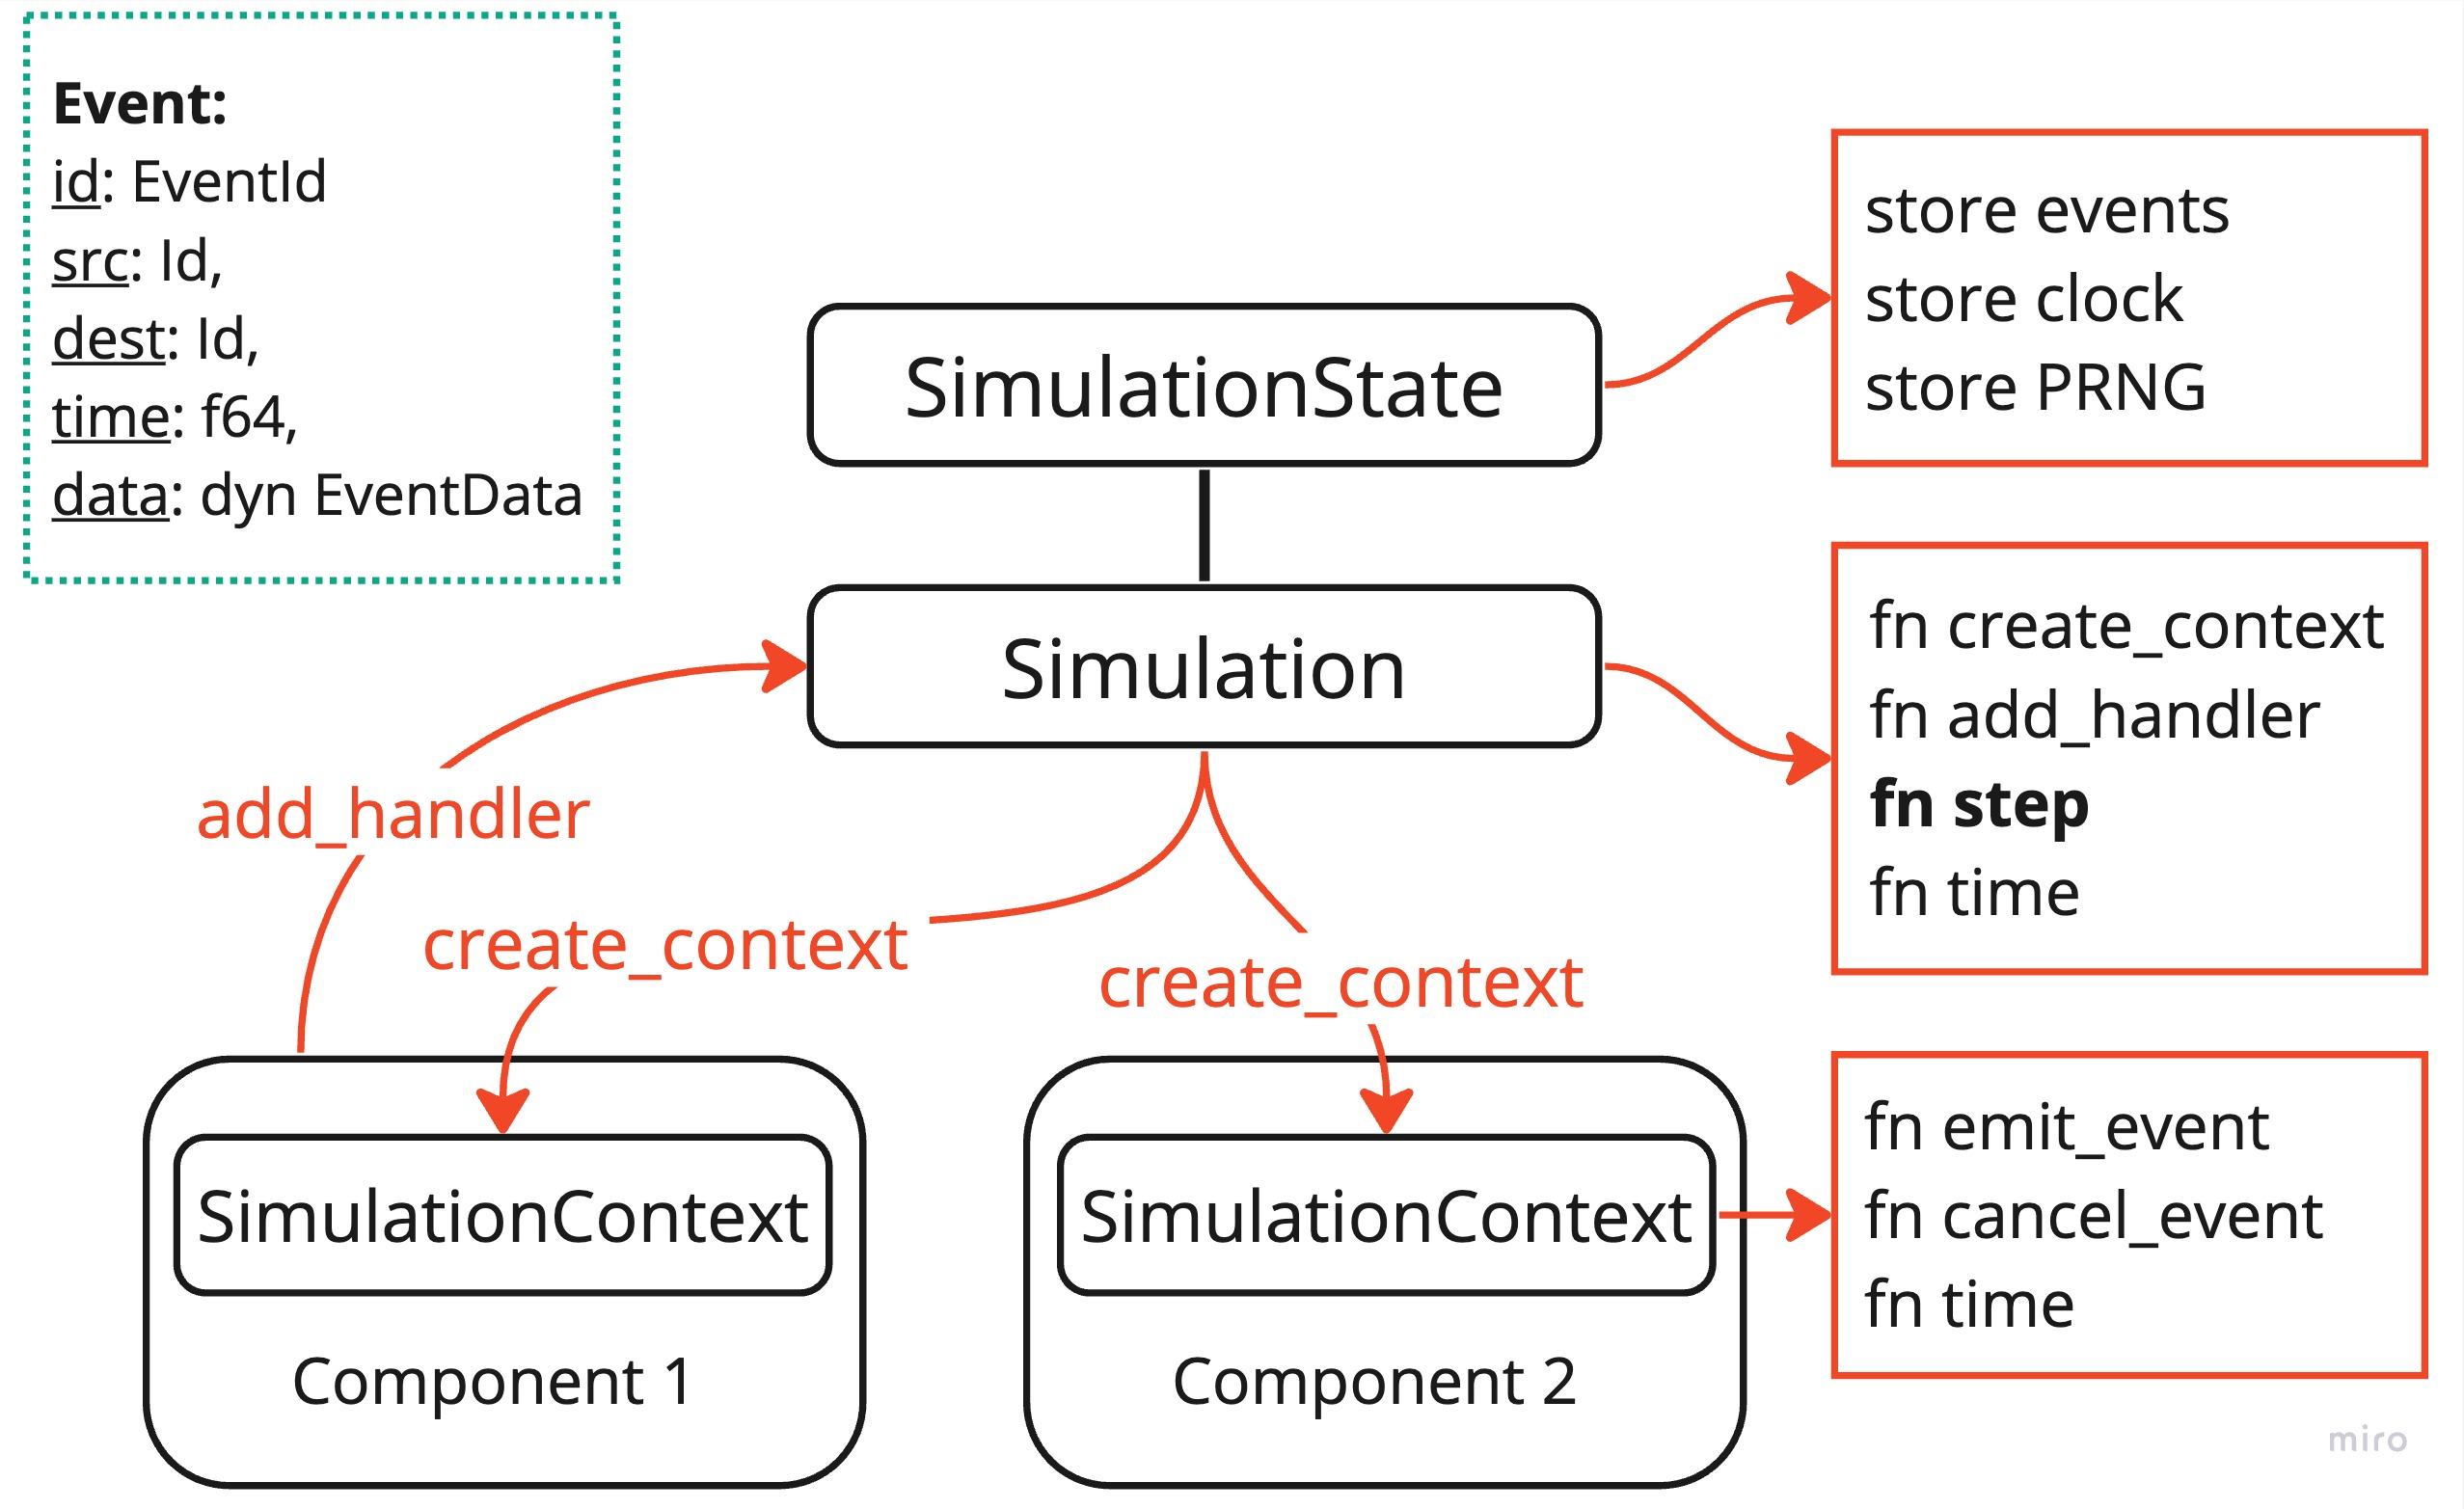
\includegraphics[width=\linewidth]{images/dslab_overview}
			\caption*{Внутреннее устройство \texttt{DSLab}}
		\end{figure}
	\end{frame}

 \section{Управление исполнением}

 \begin{frame}[fragile]
	\frametitle{\insertsection} 
	\framesubtitle{\insertsubsection}

	\begin{columns}
		\begin{column}[c]{0.45\linewidth}
			\vspace{0.5cm}
			\begin{figure}
				\centering
				\scriptsize
				\begin{rustcode}
fn on_start_action(&self) {
  // do 1
}

fn on_first_event(&self) {
  // do 2
}

fn on_second_event(&self) {
  // do 3
}
			\end{rustcode}
				\caption*{Синхронный код (разрезан на части разработчиком)}
			\end{figure}
		\end{column}
		\begin{column}[c]{0.05\linewidth}
			\vspace{0.2cm}
			$\iff$
		\end{column}
		\begin{column}[c]{0.55\linewidth}
			\vspace{0.3cm}
			\begin{figure}
				\centering
				\scriptsize
				\begin{rustcode}
async fn action(&self) {
  // do 1

  wait_for_first_event().await;

  // do 2 

  wait_for_second_event().await;

  // do 3
}
			\end{rustcode}
				\caption*{Асинхронный код (разрезан на части компилятором)}
			\end{figure}
		\end{column}
	\end{columns}
 \end{frame}

\end{document}